\chapter{Methodology} \label{ch:methodology}
    \section{Aims} \label{sec:aims}
        Extending the experiments by \cite{higgins2017beta}, we aim to make further comparisons between the $\beta$-VAE and VAE by focusing on two variables. The first experiment tests how model performance depends on the size of the encoder bottleneck with the varying $\beta$ values. The second experiment tests how how model performance depends on the data complexity, by varying the number of generative factors, with the varying $\beta$ values.
        
        The focus of the first experiment is on the relationship between the performance, latent bottleneck size and the $\beta$ values. This is an interesting question because it may be possible that when the dimension of the latent space(the bottleneck) is very close to the original number of generative factors, the role of KL divergence becomes less important. In another words, the role of the weight of the KL divergence may become more important as the latent space becomes significantly larger than that of the number of generative factors. If this hypothesis is the true, this has an important practical implication. In most real scenarios, we will not have access to the original number of generative factors of the data set. For example, how many generative factors are there for the ImageNet\citep{Deng09imagenet:a} dataset? Therefore, in most scenarios, we will have to make a safe overestimate of the number of learnable factors and set the number of latent dimensions to be generously large. Therefore, if the hypothesis is true, then in most real scenarios, the choice of $\beta$ will be important factor to consider. In order to test this, we will fix a data set with a known number of generative factors $n$. Then, starting with the bottleneck with size $n$, we will compare the two models' performances as we increase the size of the bottleneck.
        
        The second experiment compares model performance when we vary the complexity of the input data by increasing the number of generative factors. \cite{higgins2017beta} already showed some promising results that the $\beta$-VAE outperforms the standard VAE on certain data sets(celebA, 3D chairs, 3D faces, dSprites). However, it seems likely that the two models would perform similarly on extremely simple data sets, for example, if the data set only had a single position variable as the generative factor. The question then is at what level of complexity, and at what rate, do the two models' performances diverge? For this test, we will compare the model performances as we vary the complexity of the data set, by increasing the number of generative factors.
        
    \section{Data} \label{sec:data}
        The structure of the data set will be based on dSprites by \cite{dsprites17} with small differences. Firstly, dSprites has an image for every single combination of each generative factors, each of which is from a fixed finite set:
        
        \begin{itemize}
            \item Colour: white
            \item Shape: square, ellipse, heart
            \item Scale: 6 values linearly spaced in [0.5, 1]
            \item Orientation: 40 values in [0, $2\pi$]
            \item Position X: 32 values in [0, 1]
            \item Position Y: 32 values in [0, 1]
        \end{itemize}
        
        \begin{figure}[H]
            \centering
            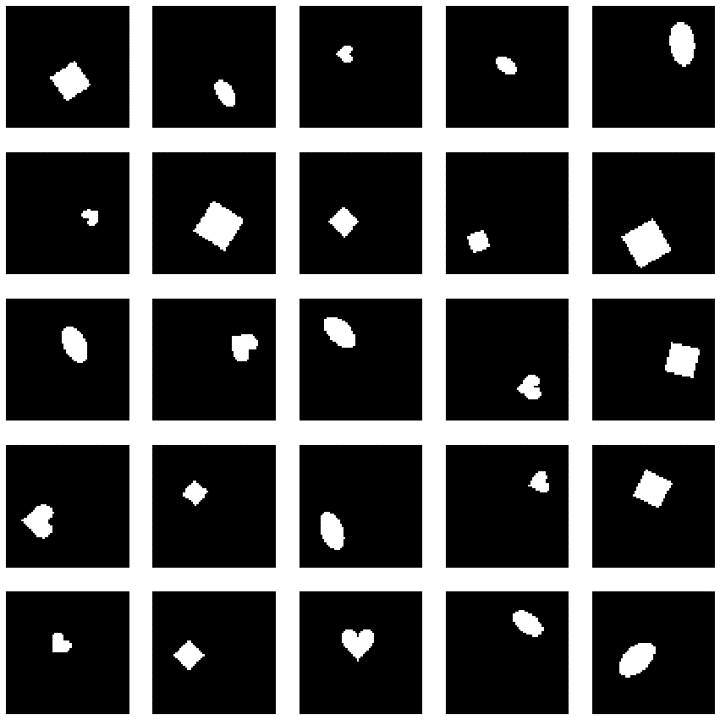
\includegraphics[width=0.5\textwidth]{imgs/dSprites.png}
            \caption{dSprites images from \cite{dsprites17}}
            \label{fig:colour_scale}
        \end{figure}
        
        This means that there are $1 \times 3 \times 6 \times 40 \times 32 \times 32 = 737280(\sim 1 \text{ million})$ images. We plan to use data sets with more generative factors but then the file size becomes impractically large. So instead of having an image for each possible combination of all the factors, we decided to have a fixed number of image set size of one million and uniformly sample each factor for each image. As well as the practicality of the file size, another advantage of this approach is that the images could have the factor values from a continuous range instead of a small predefined finite set as with dSprites. Also, even though the data set will not have an image for every single combination of the factors, this should not be too much of a problem as the generative factors are all mostly uncorrelated factors and the sample size of a million should be large enough for the model to see enough examples for each partial combination of factors. These are the factors in order that will cumulatively be added on for the increasingly complex data sets:
        
        \begin{enumerate}
            \item Position $X\sim U[0, 1]$
            \begin{center}
                
\includegraphics[width=0.7\textwidth]{imgs/1pos.png}
            \end{center}
            \item Position $Y\sim U[0, 1]$
            \begin{center}
                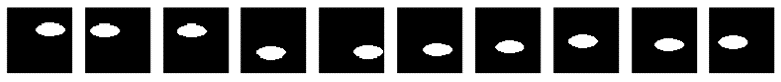
\includegraphics[width=0.7\textwidth]{imgs/2pos.png}
            \end{center}
            \item Scale $S\sim U[0, 1]$
            \begin{center}
                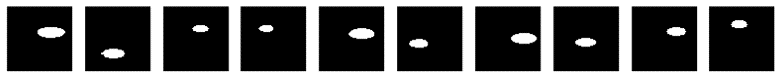
\includegraphics[width=0.7\textwidth]{imgs/2pos_scl.png}
            \end{center}
            \item Shape: square[cube], ellipse[ellipsoid], triangle[pyramid]
            \begin{center}
                
\includegraphics[width=0.7\textwidth]{imgs/2pos_scl_shape.png}
            \end{center}
            \item Rotation1: $Rotation_X\sim U[0, 2\pi]$
            \begin{center}
                
\includegraphics[width=0.7\textwidth]{imgs/2pos_scl_shape_1rot.png}
            \end{center}
            \item Colour: $HSV(h, s=1, v=1)$ where $h\sim U[0, 1]$
            \begin{center}
                
\includegraphics[width=0.7\textwidth]{imgs/2pos_scl_shape_1rot_col.png}
            \end{center}
            \item Rotation2: $Rotation_Y\sim U[0, 2\pi]$ (3D)
            \begin{center}
                
\includegraphics[width=0.7\textwidth]{imgs/2pos_scl_shape_2rot_col.png}
            \end{center}
        \end{enumerate}
        
        Note there is another minor difference of using a triangle instead of a heart as in dSprites. Also, it was a deliberate choice to choose a one dimensional colour scale by varying only the hue in HSV colour scheme:
        
        \begin{figure}[H]
            \centering
            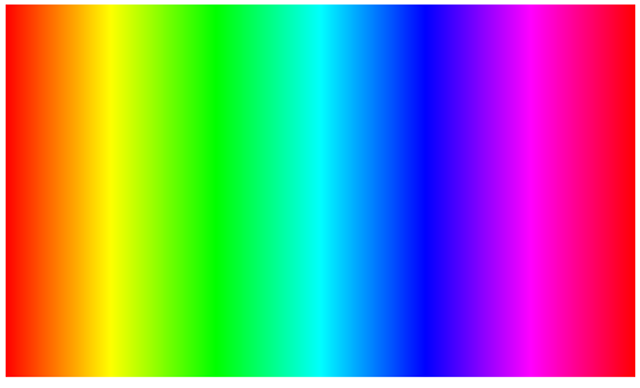
\includegraphics[width=0.5\textwidth]{imgs/colour_scale.png}
            \caption{1 dimensional colour scale based on $HSV(h, s=1, v=1)$ where $h\in[0, 1]$ }
            \label{fig:colour_scale}
        \end{figure}
        
        The reason for this choice, instead of going for the standard colour schemes such as the 3 dimensional RGB system, is that there is more than one way to represent the multidimensional colour which may lead to a model learning a perfectly valid form of a disentangled representation of colour but may not correspond to the exact system used in generating the images. This could cause problem in comparing disentanglement between models. Similarly, only two dimensions of rotation are used instead of three dimensions for the 3D data sets since there is more than one way to produce the same orientation if we use three dimensions. The two dimension of rotations should be independent enough for good comparisons.
        
    \section{Comparison criteria}
        There are two criteria we will use to compare the models. The first is the qualitative inspection of the reconstructed images in the latent space through the method of latent traversals as we already saw in figure \ref{fig:entangled_disentangled}. The second is the quantitative disentanglement metric which aims to measure how well the model encodes the independent features using separate latent dimensions. We now discuss the trade-offs of two different disentanglement metrics proposed by \cite{higgins2017beta} and \cite{kim2018disentangling}.
        
        \subsection{Disentanglement metric \citep{higgins2017beta}}
        The first proposal of a disentanglement metric was made by \cite{higgins2017beta}. In essence, a simple classifier is used to measure the one to one correspondence between the latent dimensions and the ground truth generative factors. Here are the steps from \cite{higgins2017beta}:
        
        \begin{enumerate}
            \item Randomly choose a generative factor $k \in [1,...,K]$ where $K$ is the size of the latent space dimension.
            \item For a batch of $l = 1,...,L$ samples:
                \begin{enumerate}
                    \item Sample two sets of latent vectors $\bm{v}_{1,l}$ and $\bm{v}_{2,l}$ making sure that the value of the latents in the $k^{th}$ coordinates are equal.
                    \item For each $n=1,2$, generate images $\bm{x}_{n,l}$ using the decoder of the model. Then infer $\bm{z}_{n,l} = \bm{\mu}_{\bm{x}_{n, l}}$ from the posterior distribution $N(\bm{\mu}_{\bm{x}_{n, l}}, \bm{\Sigma}_{\bm{x}_{n, l}})$ from the model's encoder.
                    \item Compute the absolute difference $\bm{z}_{diff}^l = | \bm{z}_{1,l} - \bm{z}_{2,l} |$
                \end{enumerate}
            \item Use the average $\bm{z}_{avg} = \frac{1}{L}\sum_{l=1}^L \bm{z}_{diff}^l$ to predict $p(y|\bm{z}_{avg})$.
        \end{enumerate}
        
        In the third step, \cite{higgins2017beta} used a linear classifier with low Vapnik–Chervonenkis dimension, i.e. low expressive power, to ensure that the classifier cannot do any complex non-linear disentangling itself. The diagram below illustrates these steps.
        
        \begin{figure}[H]
            \centering
            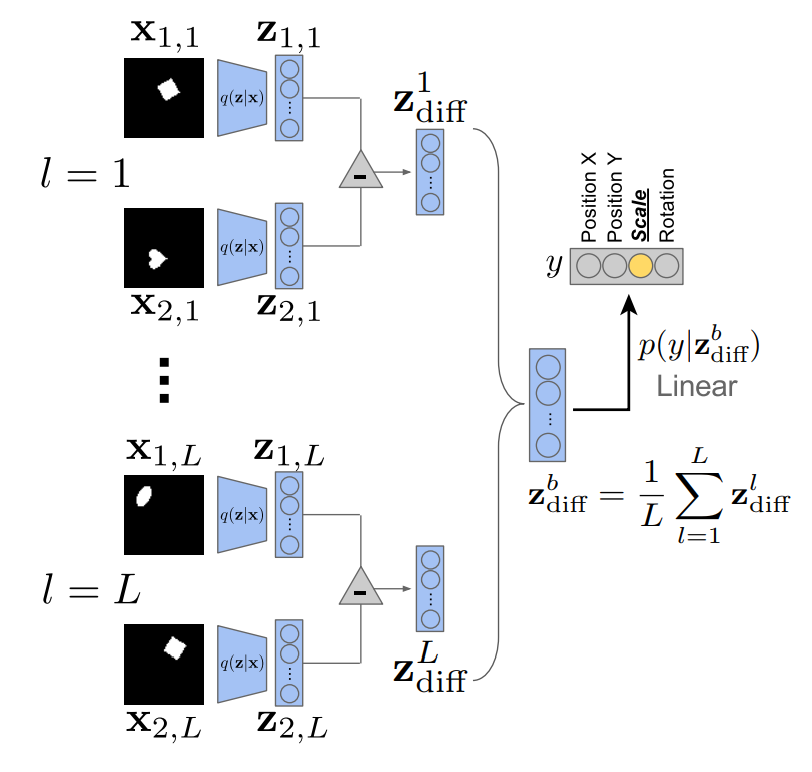
\includegraphics[width=0.4\textwidth]{imgs/disentanglement_metric_higgins.png}
            \caption{Figure from \cite{higgins2017beta}. Schematic of the disentanglement metric by \cite{higgins2017beta}}
            \label{fig:disentanglement_metric_higgins}
        \end{figure}
        
        The proposed metric serves its purpose because the model will need to produce a well disentangled latent space which makes a good one-to-one correspondence with the generative factors so that even a simple linear classifier can make high accuracy predictions as to which generative factor was held constant in the batch of samples. However, there are some limitations associated with this approach, as pointed out by \cite{kim2018disentangling}. Firstly, the metric could be sensitive to the choice of the linear classifier used, the hyperparameters, the weight initialisations, and the optimiser used for the classifier. Secondly, even if it's true that the linear classifier cannot make complex non-linear predictions, even a linear combination of the latent dimensions may in some cases be strong enough to do its own disentanglement which defeats the purpose of measuring disentanglement. Thirdly, this metric is computationally expensive since each new measurement of disentanglment requires training a new classifier. This is not ideal especially if one needs to calculate the metric thousands of times. Lastly, there are scenarios in which the metric gives a misleading score. Using the example by \cite{kim2018disentangling}, suppose we have a data set with 4 generative factors: x-position, y-position, scale and shape. Suppose the model has perfectly learned disentangled representations of the first three of the generative factors but has not learned shape. In this scenario, the linear classifier undesirably gives a disentangled metric score of 100\% as the linear classifier can "correctly" predict that when the other latents' values corresponding to the first three generative factors are non-zero, it must be the last unlearnt factor which was kept constant.
        
        \begin{figure}[H]
            \centering
            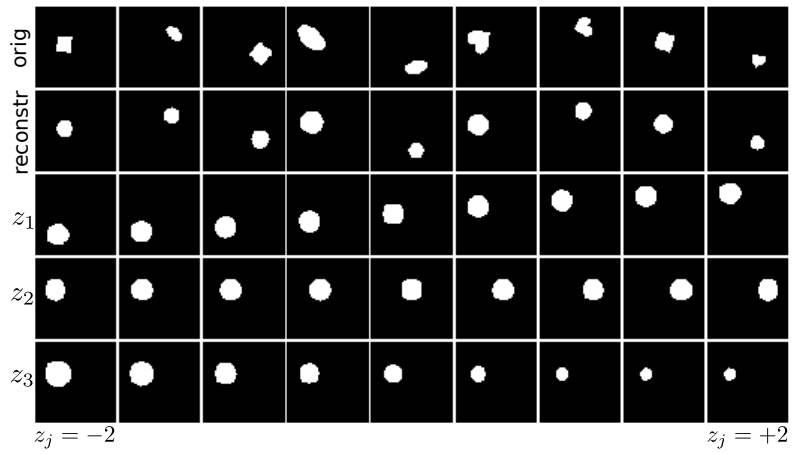
\includegraphics[width=0.4\textwidth]{imgs/counter_example_kim.png}
            \caption{Figure from \cite{kim2018disentangling}. A setting in which the metric by \cite{higgins2017beta} incorrectly gives a 100\% score without perfect disentanglement.}
            \label{fig:counter_example_kim}
        \end{figure}
        
    \subsection{Disentanglement metric \citep{kim2018disentangling}} \label{subsec:metric_kim}
        To address these limitations, \cite{kim2018disentangling} propose a new metric. However, there is one key extra assumption that is required for this metric to work, which is that we need the full access to the ground truth image generator with which we can fully control of the generative features when generating the images. Of course, this is an unhelpful assumption for real life data sets but it can be a useful for experimenting with synthetic data sets as with this project.
        
        \begin{enumerate}
            \item Randomly choose a generative factor $k \in [1,...,K]$ where $K$ is the size of the latent space dimension.
            \item For a batch of $l = 1,...,L$ samples:
                \begin{enumerate}
                    \item Generate images $\bm{x}_l$ with the $k^{th}$ generative factor fixed.
                    \item Infer $\bm{z}_l = \bm{\mu}_{\bm{x}_l}$ from the posterior distribution $N(\bm{\mu}_{\bm{x}_l}, \bm{\Sigma}_{\bm{x}_l})$ from the model's encoder.
                    \item Normalise each dimension by its empirical standard deviation over the full data(or a large enough subset).
                \end{enumerate}
            \item The index $d \in [1,...,D]$ of the normalised latent dimensions with the lowest variance, together with $k$, provide one training $(d,k)$ = (input, output) example for the majority vote classifier. The accuracy of the classifier is the final disentanglement score.
        \end{enumerate}
        
        The normalisation at step 2.c) is to ensure that the minimum index is invariant of the rescaling of of the representations in each dimension. The majority vote classifier $C$ used in the third step is defined as follows:
        
        \begin{itemize}
            \item Begin with a training set $(d_m, k_m)$ for $m in [1,...,M]$, where $M$ is the fixed size of the training set, $d=1,...,D$ where $D$ is the number of the latent dimensions, and $K$ is the number of the generative factors.
            \item Then for each $d \in [1,...,D]$ and $k \in [1,...,K]$, calculate $V_{d,k} = \sigma_{m=1}^M \mathbb{I}(d_m = d, k_m = k)$
            \item Finally, our classifier $C$ is defined by the equation: $C(d) = \operatorname*{argmin}_k V_{d, k}$.
        \end{itemize}
        
        Note that $D$ does not affect the metric because, for example, if the classifier chose at random, the accuracy would be $\frac{1}{K}$ independent of $D$.
        
        \cite{kim2018disentangling} explains that this approach addresses the problems faced by the metric by \cite{higgins2017beta}. Firstly, the majority vote classifier used for this metric is completely deterministic without the need for a choice of hyperparameters etc. Secondly, since the classifier is a simple majority vote, there is no room for any further disentanglement in calculating the score, even linear combinations between the latent dimensions. Thirdly, the classifier only needs to do simple counts to train, which significantly reduces the computation time. Finally, since the classifier needs to see the lowest variance in a latent dimension for a given factor to classify correctly, it avoids making misleading scores unlike the previous metric.
        
    \section{Model architectures}
        Below is the full model architectures used for this project:
        
        \begin{itemize}
            \item Neural Network
            \begin{center}
                \begin{tabular}{| c | c |}
                    \multicolumn{2}{c}{\textbf{Encoder}}\\
                    \hline
                    \multicolumn{2}{|c|}{\textbf{Input} $\bm{x}_{in}$: $64 \times 64 \times C$(Channels)}\\
                    \hline
                    \multicolumn{2}{|c|}{$4 \times 4$ conv. 32 ReLU. stride 2}\\
                    \hline
                    \multicolumn{2}{|c|}{$4 \times 4$ conv. 32 ReLU. stride 2}\\
                    \hline
                    \multicolumn{2}{|c|}{$4 \times 4$ conv. 32 ReLU. stride 2}\\
                    \hline
                    \multicolumn{2}{|c|}{$4 \times 4$ conv. 32 ReLU. stride 2}\\
                    \hline
                    \multicolumn{2}{|c|}{FC. 256 ReLU}\\
                    \hline
                    \multicolumn{2}{|c|}{FC. 256 ReLU}\\
                    \hline
                    $\bm{\mu}$: FC. $D$(Latent size) & $\bm{\Sigma}$: FC. $D$(Latent size) \\
                    \hline
                    \multicolumn{2}{c}{}\\
                    \multicolumn{2}{c}{\textbf{Sampler}}\\
                    \hline
                    \multicolumn{2}{|c|}{\textbf{Sample} $\bm{z}: \bm{\mu} + \bm{\Sigma} \odot \bm{\epsilon}$ where $\bm{\epsilon} \sim N(\bm{0},\bm{I})$}\\
                    \hline
                    \multicolumn{2}{c}{}\\
                    \multicolumn{2}{c}{\textbf{Decoder}}\\
                    \hline
                    \multicolumn{2}{|c|}{\textbf{Input}: $D$}\\
                    \hline
                    \multicolumn{2}{|c|}{FC. 256 ReLU}\\
                    \hline
                    \multicolumn{2}{|c|}{FC. 512 ReLU}\\
                    \hline
                    \multicolumn{2}{|c|}{$4 \times 4$ deconv. 32 ReLU. stride 2}\\
                    \hline
                    \multicolumn{2}{|c|}{$4 \times 4$ deconv. 32 ReLU. stride 2}\\
                    \hline
                    \multicolumn{2}{|c|}{$4 \times 4$ deconv. 32 ReLU. stride 2}\\
                    \hline
                    \multicolumn{2}{|c|}{$4 \times 4$ deconv. 32 ReLU. stride 2}\\
                    \hline
                    \multicolumn{2}{|c|}{\textbf{Output} $\bm{x}_{out}$: $64 \times 64 \times C$(Channels)}\\
                    \hline
                \end{tabular}
            \end{center}
                
            \item Number of input channels $C$: 1(BW) or 3(RGB)
            
            \item Dimensionality of the latent space $D$:
            \begin{itemize}
                \item Experiment 1:\\
                For the first experiment as defined in section \ref{sec:aims}, we will vary $D$ on the fixed data set with the first 5 generative factors as defined in section \ref{sec:data}. Since we have 5 generative factors, we will vary $D$ starting with 5 up to 20 in increments of 5.
                
                \item Experiment 2:\\
                For the second experiment, we will keep $D=20$ fixed which is safely larger than the maximum number of generative factors used in this project which is 7.
            \end{itemize}
            
            \item Batch size: 64(fixed)
            
            \item Learning rate: 0.0005(fixed)
            
            \item Optimiser: Adam(fixed)
            
            \item Loss function: $\mathbb{E}_{q_{\bm{\theta_x}}(\bm{z}|\bm{x})} \left[\log p(\bm{x} | \bm{z}) \right] + \beta KL\left[q_{\bm{\theta_x}}(\bm{z}|\bm{x}) || p(\bm{z})\right]$(fixed)
            
            \item Hyperparameter $\beta$: 1, 2, 4, 8
            
            \item Max epochs:
            \begin{itemize}
                \item 1 \& 2 generative factors: 10 epochs
                \item 3 generative factors: 20 epochs
                \item 4 \& 5 generative factors: 30 epochs
                \item 6 \& 7 generative factors: 60 epochs
            \end{itemize}
            
        \end{itemize}